\documentclass[11pt]{article} % use larger type; default would be 10pt


%%% PAGE DIMENSIONS
\usepackage[top=1in, bottom=1in, left=1in, right=1in]{geometry} % to change the page dimensions
 
%%% PACKAGES
\usepackage{graphicx} % support the \includegraphics command and options
\usepackage{amsfonts}
\usepackage{amsmath}
\usepackage{tikz}
\usepackage{graphicx}


%%% The "real" document content comes below...

\title{CS 134 \\ \emph{Problem Set 2}}
\author{Xiner Zhou}
\date{\today} % Activate to display a given date or no date (if empty),
        

\begin{document}
 
\maketitle

\paragraph{1. The square lattice. (20 points)}

\begin{enumerate}

\item[\textbf{a.}] \textbf{(6 points)}  
The pairs of nodes in a square lattice that are farthest apart (i.e. largest lattice distance) must be those that are located on the diagonals, say A and B, and they have $2(r-1)=2(\sqrt{n}-1)$ lattice distance apart, givcen that there exist short-cuts between every pair of nodes that are two lattice distance apart, the shortest path between A and B has length $\frac{2(r-1)}{2}=\frac{2(\sqrt{n}-1)}{2}=\sqrt{n}-1$. Therefore, the diameter of a 2-square lattice on n nodes is $\sqrt{n}-1$.

\item[\textbf{b.}] \textbf{(8 points)}  
Consider a node $u=(i,j)$ that is at lattice distance at least 2 from any nodes on the edge of the lattice, the number of nodes that are d lattice distance away from $u$ is $4d$. Therefore, the total number of neighbors $u$ has is: $$ |N(u)|=\sum \limits_{d=1}^{2} 4d=4+8=12 $$

Now, let's calculate the number of edges among neighbors of $u$, i.e., how many neighbors of $u$ are themselves neighbors. We observe that, the nodes that are 1 hop away from $u$, i.e., $(i-1,j),(i,j-1),(i+1,j),(i,j+1)$ each has 6 neighbors in $N(u)$; among the nodes that are 2 hops away from $u$, $(i-2,j),(i+2,j),(i,j-2),(i,j+2)$, each has 3 neighbors in $N(u)$; among the nodes that are 2 hops away from $u$, $(i+1,j+1),(i-1,j-1),(i-1,j+1),(i+1,j-1)$ each has 6 neighbors in $N(u)$. Therefore, the total number of edges in $N(u)$ is: $$\frac{4(6+3+6}{2}=30$$

The clustering coefficient of a node $u$ is: $$\displaystyle{ c(u)= \frac{30}{\frac{12!}{10! 2!}}=\frac{5}{11}}$$

\item[\textbf{c.}] \textbf{(6 points)} 

\begin{center}
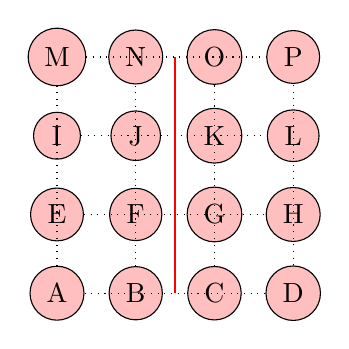
\begin{tikzpicture}[node distance=1.5cm, scale=1]

\node[draw, shape=circle, fill=pink] (n1) at (0,0) {A};
\node[draw, shape=circle, fill=pink] (n2) at (1,0) {B};
\node[draw, shape=circle, fill=pink] (n3) at (2,0) {C};
\node[draw, shape=circle, fill=pink] (n4) at (3,0) {D};

\node[draw, shape=circle, fill=pink] (n5) at (0,1) {E};
\node[draw, shape=circle, fill=pink] (n6) at (1,1) {F};
\node[draw, shape=circle, fill=pink] (n7) at (2,1) {G};
\node[draw, shape=circle, fill=pink] (n8) at (3,1) {H};

\node[draw, shape=circle, fill=pink] (n9) at (0,2) {I};
\node[draw, shape=circle, fill=pink] (n10) at (1,2) {J};
\node[draw, shape=circle, fill=pink] (n11) at (2,2) {K};
\node[draw, shape=circle, fill=pink] (n12) at (3,2) {L};

\node[draw, shape=circle, fill=pink] (n13) at (0,3) {M};
\node[draw, shape=circle, fill=pink] (n14) at (1,3) {N};
\node[draw, shape=circle, fill=pink] (n15) at (2,3) {O};
\node[draw, shape=circle, fill=pink] (n16) at (3,3) {P};

 
 

\draw[-, dotted] (n1) to (n4);
\draw[-, dotted] (n5) to (n8);
\draw[-, dotted] (n9) to (n12);
\draw[-, dotted] (n13) to (n16);

\draw[-, dotted] (n1) to (n13);
\draw[-, dotted] (n2) to (n14);
\draw[-, dotted] (n3) to (n15);
\draw[-, dotted] (n4) to (n16);
  
\draw[-, thick, color=red] (1.5,0 ) to (1.5, 3);

\end{tikzpicture}
\end{center}

For even $r$, we could cut the square lattice as the above example shows, which cuts the graph into equal halves. For this kind of cut, we find a set of nodes $S$ of size equal to $\frac{n}{2}$ has $r=\sqrt{n}$ edges leaving it, so by definition, the expansion parameter of the graph is smaller or equal to $\frac{r}{\frac{n}{2}}=\frac{\sqrt{n}}{\frac{n}{2}}=\frac{2}{\sqrt{n}}=\frac{2}{r}$. 

\end{enumerate}


\paragraph{2. A smaller world? (Easley and Kleinberg, 20.8 Q1) (20 points)}   
We can use a k-square lattice on n nodes, where n is the full population of the world, and the lattice distance us a "closeness" or "friendship" measures that basically quantifies how close each pair of people are. For every node in the lattice, we create an edge to their closest 10 nodes in the lattice distance. 

Notice that in a 2-square lattice, each node already has 12 neighbors, and in a 1-square lattice, each node has only 4 neighbors, therefore, the graph we are generating for the "close-friend" is less connected than a 2-square lattice, it should be somewhere between 1- and 2-square lattice.

From \textbf{1 a.}, we know that for $k=2$, the diameter of the 2-square lattice is $\sqrt{n}-1$. And we can easily observe that  for 1-square lattice, the diameter is $2(\sqrt{n}-1)$. Therefore, the "close-friend" network should have a diameter proportional to $\sqrt{n}$, or $\Theta(\sqrt{n})$. Since $n$ is the total population of the world, $\sqrt{n}$ is far much greater than 6. It's equivalent to say that there exists at least a pair of people in the world, that the path connecting requires at least $\Theta(\sqrt{n})$ steps. 

In conclusion, it is impossible that for each pair of people in the world, there is a path of at most six edges connecting this pair of people.

\paragraph{3. Keep your friends close, and your acquaintances closer. (Easley and Kleinberg, 20.8 Q2) (20 points)}  
 
\begin{enumerate}

\item[\textbf{a.}]  \textbf{(8 points)} 
I expect the close-friend network to have the largest clustering coefficient. 

To think about clustering coefficients, we are essentially talking about the principle of triadic closure: If two people in a social network have a friend in common, then there is an increased likelihood that they will become or already are friends themselves. The supporting arguments are based on opportunity, trust, and incentives. And furthermore, the likelihood of triadic closure are more powerful when the edges are srong ties (in this case, top 10 closest friends) than when they are weak ties (equivalent to 21-30 friends).

\item[\textbf{b.}]  \textbf{(8 points)}  
I expect to see the "long-range" edges in distant-friend networks. 

In the Watts-Strongatz model and the Kleinberg model, the lattice distance represent some kind of notion of similarity that guides the formation of the links. It could be geographic proximity or social proximity. By definition, for any people, we denote it as $u$ in the graph, the 10 closest friends are more likely (or certainly) have small distance away from $u$, while the 21-30 friends are more likely to be not so much alike $u$, therefore, are more likely to have "long-range" edges away from $u$.


\item[\textbf{c.}]  \textbf{(4 points)}
I expect $D$ to be larger. 

As I indicated in \textbf{3 a.}, close-friend network (strong ties) tend to have larger clustering coefficient than the distant-friend network (weak ties), that is to say, close-friend network has more triangles -- sets of three people who mutually know each other. As a result, in each branching step, the number of nodes a person can reach in a close-friend network is less than that in a distant-friend network, because many of these edges go from one friend to another, not to the rest of the workld, in a close-friend network. Therefore, the average number of people that a person can reach in six steps in the distant-friend network should be expected to be larger.

\end{enumerate}
 

\paragraph{4. Regular graphs. (20 points)}  

\begin{enumerate}

\item[\textbf{a.}]\textbf{(6 points)}  

A ring lattice with n=12 nodes and k=1. Justifications:
\begin{itemize}
\item Each pair of nodes has a path connecting them, and each node has 2 edges, so it is a connected 2-regular graph.
\item The longest distance is between the nodes on the opposite side of a diameter, which is $\frac{n}{2}$. Therefore, the diameter is $\frac{n}{2}$. 
\item There is no triadic closure, so the clustering coefficient of the graph is 0.
\end{itemize}

\begin{center}
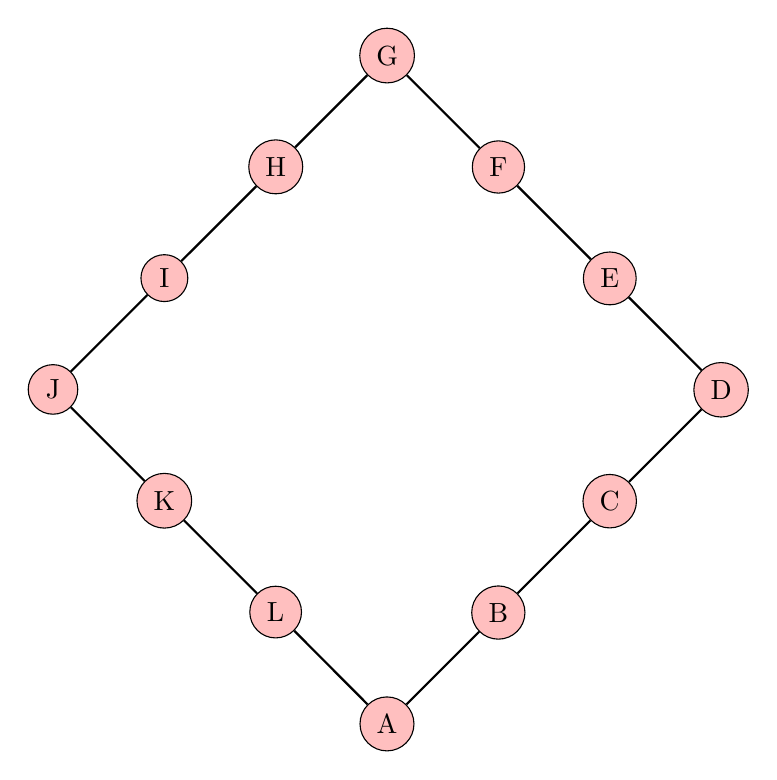
\begin{tikzpicture}[node distance=2cm, scale=1.5]

\node[draw, shape=circle, fill=pink] (n1) at (0,0) {A};
\node[draw, shape=circle, fill=pink] (n2) [above right of =n1] {B};
\node[draw, shape=circle, fill=pink] (n3) [above  right of =n2] {C};
\node[draw, shape=circle, fill=pink] (n4) [above right  of =n3] {D};
\node[draw, shape=circle, fill=pink] (n5) [above left of =n4] {E};
\node[draw, shape=circle, fill=pink] (n6) [above left of =n5] {F};

\node[draw, shape=circle, fill=pink] (n7) [above left of =n6] {G};
\node[draw, shape=circle, fill=pink] (n8) [below left of =n7] {H};
\node[draw, shape=circle, fill=pink] (n9) [below left of =n8] {I};
\node[draw, shape=circle, fill=pink] (n10) [below left of =n9] {J};
\node[draw, shape=circle, fill=pink] (n11) [below right of =n10] {K};
\node[draw, shape=circle, fill=pink] (n12) [below right of =n11] {L};
 

\draw[-, thick] (n1) to (n2);
\draw[-, thick] (n2) to (n3);
\draw[-, thick] (n3) to (n4);
\draw[-, thick] (n4) to (n5);
\draw[-, thick] (n5) to (n6);
\draw[-, thick] (n6) to (n7);
\draw[-, thick] (n7) to (n8);
\draw[-, thick] (n8) to (n9);
\draw[-, thick] (n9) to (n10);
\draw[-, thick] (n10) to (n11);
\draw[-, thick] (n11) to (n12);
\draw[-, thick] (n12) to (n1);
 

\end{tikzpicture}
\end{center}


\item[\textbf{b.}] \textbf{(14 points)}  

A ring lattice with n=12 nodes and k=2. Justifications:
\begin{itemize}
\item Each pair of nodes has a path connecting them, and each node has 4 edges, so it is a connected 4-regular graph.
\item The longest distance is between the nodes on the opposite side of a diameter, which is $\frac{n}{2}$. And since each pair of nodes that are 2 hops away are connected, the distance between them is $\frac{n}{4}$.  Therefore, the diameter is $\frac{n}{4}$. 
\item For a node in the graph $u$, it has 4 neighbors, and only 3 pairs of its neighbors are themselves connected, therefore, the clustering coefficient for $u$ is: $$C(u)=\frac{3}{\frac{4!}{2!(4-2)!}}=\frac{1}{2}$$ The clustering coefficient is the same for all nodes in the graph, so the clustering coefficent of the graph is also $\frac{1}{2}$.
\end{itemize}


\end{enumerate}

\begin{center}
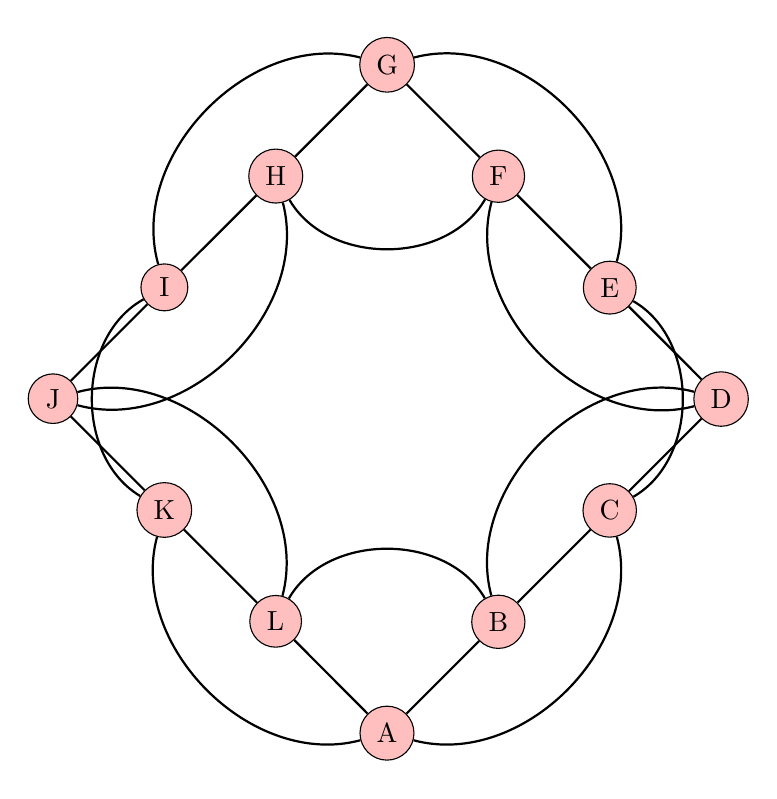
\begin{tikzpicture}[node distance=2cm, scale=1.5]

\node[draw, shape=circle, fill=pink] (n1) at (0,0) {A};
\node[draw, shape=circle, fill=pink] (n2) [above right of =n1] {B};
\node[draw, shape=circle, fill=pink] (n3) [above  right of =n2] {C};
\node[draw, shape=circle, fill=pink] (n4) [above right  of =n3] {D};
\node[draw, shape=circle, fill=pink] (n5) [above left of =n4] {E};
\node[draw, shape=circle, fill=pink] (n6) [above left of =n5] {F};

\node[draw, shape=circle, fill=pink] (n7) [above left of =n6] {G};
\node[draw, shape=circle, fill=pink] (n8) [below left of =n7] {H};
\node[draw, shape=circle, fill=pink] (n9) [below left of =n8] {I};
\node[draw, shape=circle, fill=pink] (n10) [below left of =n9] {J};
\node[draw, shape=circle, fill=pink] (n11) [below right of =n10] {K};
\node[draw, shape=circle, fill=pink] (n12) [below right of =n11] {L};
 

\draw[-, thick] (n1) to (n2);
\draw[-, thick] (n2) to (n3);
\draw[-, thick] (n3) to (n4);
\draw[-, thick] (n4) to (n5);
\draw[-, thick] (n5) to (n6);
\draw[-, thick] (n6) to (n7);
\draw[-, thick] (n7) to (n8);
\draw[-, thick] (n8) to (n9);
\draw[-, thick] (n9) to (n10);
\draw[-, thick] (n10) to (n11);
\draw[-, thick] (n11) to (n12);
\draw[-, thick] (n12) to (n1);
 
%2 hops away connections
\draw[-, thick] (n1) to [bend right=60] (n3);
\draw[-, thick] (n2) to [bend left=60] (n4);
\draw[-, thick] (n3) to [bend right=60] (n5);
\draw[-, thick] (n4) to [bend left=60] (n6);
\draw[-, thick] (n5) to [bend right=60] (n7);
\draw[-, thick] (n6) to [bend left=60] (n8);
\draw[-, thick] (n7) to [bend right=60] (n9);
\draw[-, thick] (n8) to [bend left=60] (n10);
\draw[-, thick] (n9) to [bend right=60] (n11);
\draw[-, thick] (n10) to [bend left=60] (n12);
\draw[-, thick] (n11) to [bend right=60] (n1);
\draw[-, thick] (n12) to [bend left=60] (n2);

\end{tikzpicture}
\end{center}





\paragraph{5. Coding: short distances in networks. (20 points)}  

\begin{itemize}
\item (7 points) For $r = 1, 2, \ldots, 10$ (or $n = 1, 4, \ldots, 100$), generate networks according to the Watts-Strogatz model with $k = 2$ and $l = 2$. Plot the average distance between any two nodes as a function of $n$ and plot the function $\log n$;

\begin{center}
\includegraphics[width=5in]{Q5a.png}
\end{center}

\item (6 points) For $n = 1, \ldots, 100$, generate networks according to the Kleinberg model with $k = 2$ and $l = 2$. Plot the average distance between any two nodes as a function of $n$ against $\log^2 n$;

\begin{center}
\includegraphics[width=5in]{Q5b.png}
\end{center}

\item (7 points) Compute a \textbf{good estimate} (note: this does not need to be exact; clever solutions that provide good approximations of the shortest path are preferable to brute-force solutions) of the average shortest distances of these graphs.

Original network is too large for the Floyd-Warshall aogorithm to work through efficiently. Therefore, I sample 100 nodes from the network, and make a sample subgraph, which should be a good estimate.The average distance (calculated by sampling) in the enron network and the epinions network are both infinity, that is, they are not connected. However, the livejournal network is too large to run on my computer. Please see my python notebook for details. 


\end{itemize}


\end{document}
